\begin{table*}[t]
  \centering
  \caption{Performance comparison between Tiny ViT and CNN models across different datasets}
  \label{tab:results}
  \sisetup{table-format=2.2}
  \begin{tabular}{@{} l l *{5}{S} @{}}
    \toprule
    \textbf{Dataset} & \textbf{Model} & \textbf{Accuracy} & \textbf{F1} & \textbf{Recall} & \textbf{MCC} & \textbf{Precision} \\
    \midrule

    \multirow{2}{*}{CIFAR-10}
    & \textbf{Tiny ViT} & \textbf{82.59} & \textbf{82.43} & \textbf{82.59} & \textbf{80.70} & \textbf{82.76} \\
    & CNN & 80.67 & 80.55 & 80.67 & 78.53 & 80.56 \\

    \multirow{2}{*}{CIFAR-100}
    & \textbf{Tiny ViT} & \textbf{59.40} & \textbf{59.04} & \textbf{59.40} & \textbf{59.00} & \textbf{60.00} \\
    & CNN      & 46.13 & 44.57 & 46.13 & 45.61 & 45.61 \\

    \multirow{2}{*}{STL-10}
    & Tiny ViT & 64.27 & 64.30 & 64.27 & 60.47 & 66.13 \\
    & \textbf{CNN}      & \textbf{68.36} & \textbf{68.10} & \textbf{68.36} & \textbf{64.95} & \textbf{68.78} \\
    \bottomrule
  \end{tabular}

  \vspace{0.2cm}
  \small Note: All values are percentages (\%). Bold indicates best performance in category.
\end{table*}

\section{Results}
In this chapter, the results of the experiments conducted are presented. The chapter discusses the evaluation metrics used to measure the performance of the model and the results obtained from the experiments.

\subsection{Evaluation Metrics}
These metrics will be used to show the effectiveness of the approaches proposed.

\textbf{Accuracy score}

Accuracy is a proportion of correct predictions, considering both true positives and true negatives, among a total number of samples. The formula used to calculate accuracy is the following:
\begin{equation}
  \frac{\text{TP} + \text{TN}}{\text{TP} + \text{TN} + \text{FP} + \text{FN}}
\end{equation}
where \textbf{TP} is a number of true positives, \textbf{TN} is a number of true negatives, \textbf{FP} is a number of false positives and \textbf{FN} is a number of false negatives.

\textbf{Precision score}

Precision is the ability of a classifier not to label as positive a sample that is negative. The formula used to calculate precision is the following:
\begin{equation}
  \frac{\text{TP}}{\text{TP} + \text{FP}}
\end{equation}

\textbf{Recall score}

Recall is the ability of a classifier to find all the positive samples. The formula used to calculate the recall is the following:
\begin{equation}
  \frac{\text{TP}}{\text{TP} + \text{FN}}
\end{equation}

\textbf{F1 score}

F1 score is a harmonic mean of precision and recall. The formula used to calculate the F1 score is the following:
\begin{equation}
  \frac{ 2 \times (\text{precision} \times \text{recall})}{\text{precision} + \text{recall}}
\end{equation}

\textbf{Matthews correlation coefficent}

Matthews correlation coefficent (or $\varphi$ coefficient) takes into account true and false positives and negatives and is regarded as a balanced measure that can be used even if the classes are of very different sizes. Formula used to calculate $\varphi$ coefficient is as follows:
\begin{equation}
  \frac{\text{TP} \times \text{TN} - \text{FP} \times \text{FN}}{\sqrt{(\text{TP} + \text{FP})(\text{TP} + \text{FN})(\text{TN} + \text{FP})(\text{TN} + \text{FN})}}
\end{equation}

\subsection{Results}

All models were trained for 100 epochs using a batch size of 64, with an AdamW optimizer configured with a learning rate of 3e-4 and a weight decay of 0.05. The loss function used was cross-entropy loss with label smoothing of 0.1.

Table \ref{tab:results} presents the performance comparison between the Tiny ViT and CNN models across different datasets. The following comments can be made based on the results:
\begin{enumerate}
  \item On \textbf{CIFAR-10}, Tiny ViT slightly outperformed CNN, achieving 82.59\% accuracy vs. 80.67\%. It also had a higher F1 score, recall, and MCC, indicating better generalization. The precision advantage (82.76 vs. 80.56) suggests Tiny ViT made fewer false positives.
  \item For \textbf{CIFAR-100}, Tiny ViT performed significantly better (59.40\% accuracy vs. 46.13\% for CNN). The gap was consistent across F1 score, recall, and MCC, indicating Tiny ViT handled the increased class complexity better. A notable precision boost (60.00 vs. 45.61) further supports its robustness in classification.
  \item On \textbf{STL-10}, CNN outperformed Tiny ViT (68.36\% accuracy vs. 64.27\%). The CNN model had better F1, recall, and MCC. The larger image size in STL-10 might explain why CNN performed better, as its hierarchical feature extraction could be more effective than Tiny ViT’s attention based mechanism.
\end{enumerate}

Figure \ref{fig:conf-10} and Figure \ref{fig:conf-100} show the confusion matrices for CIFAR-10 and CIFAR-100 datasets, respectively. The confusion matrices provide a visual representation of the model's performance across different classes. The diagonal elements represent the number of correctly classified instances for each class, while off diagonal elements indicate misclassifications. The confusion matrices show that Tiny ViT performed well across most classes, with a few exceptions where it struggled to distinguish between similar classes.
\begin{figure}[!ht]
  \centering
  \begin{subfigure}[t]{0.48\columnwidth}
      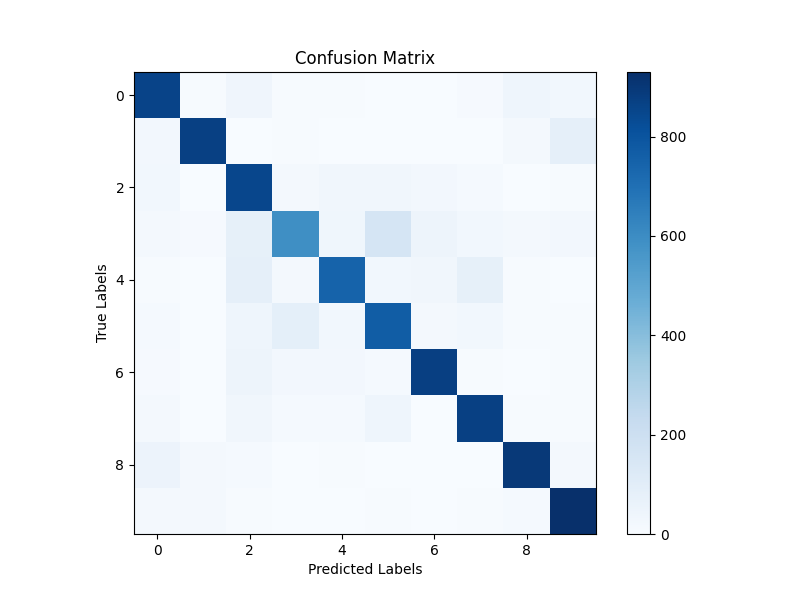
\includegraphics[width=\textwidth]{./images/cm_vit_cifar10.png}
      \caption{Confusion Matrix for CIFAR-10 dataset using Tiny ViT}
      \label{fig:conf-10}
  \end{subfigure}
  \hfill
  \begin{subfigure}[t]{0.48\columnwidth}
      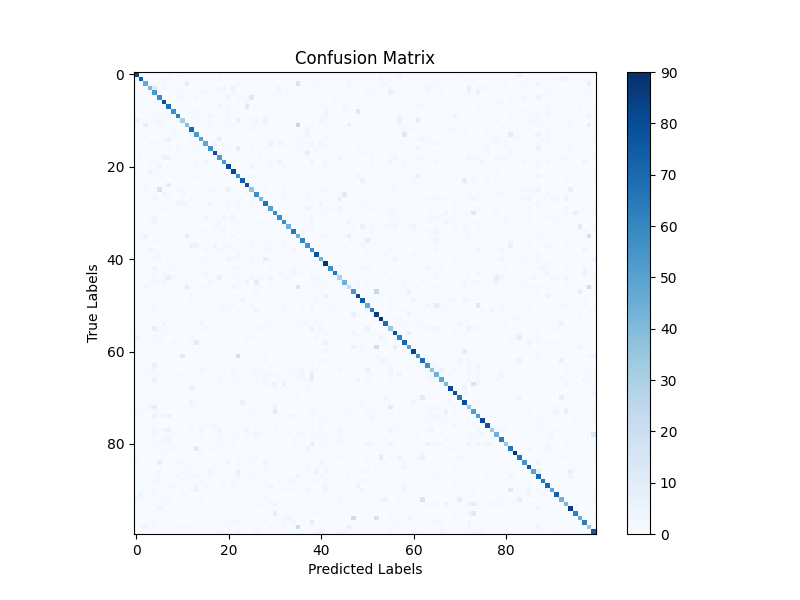
\includegraphics[width=\textwidth]{./images/cm_vit_cifar100.png}
      \caption{Confusion Matrix for CIFAR-100 dataset using Tiny ViT}
      \label{fig:conf-100}
  \end{subfigure}
\end{figure}

Overall, Tiny ViT showed clear advantages in CIFAR-10 and CIFAR-100, particularly in handling complex class distributions, while CNN performed better on STL-10, possibly due to its ability to capture local features in higher resolution images.